%%%%%%%%%%%%%%%%%%%%%%%%%%%%%%%%%%%%%%%%%%%%%%%%%%%%%%%%%%%%%%%%%%%%%%%%
% Beamer Presentation - LaTeX - Template Version 1.0 (10/11/12)
% This template has been downloaded from: http://www.LaTeXTemplates.com
% License: % CC BY-NC-SA 3.0 (http://creativecommons.org/)
% Modified by Rahmat M. Samik-Ibrahim
% REV346 Sun 12 Sep 2021 17:00:19 WIB
% REV319 Mon 19 Jul 2021 23:57:40 WIB
% REV239 Sun Sep 13 19:17:17 WIB 2020
% REV195 Wed Feb 20 20:03:01 WIB 2019
% REV119 Tue Feb 20 08:47:10 WIB 2018
% STARTX Wed Sep 14 10:46:00 WIB 2016
%%%%%%%%%%%%%%%%%%%%%%%%%%%%%%%%%%%%%%%%%%%%%%%%%%%%%%%%%%%%%%%%%%%%%%%%%

% PACKAGES AND THEMES ZCZC
\documentclass[xcolor=table, notheorems, hyperref={pdfpagelabels=false}]{beamer}
%%%%%%%%%%%%%%%%%%%%%%%%%%%%%%%%%%%%%%%%%%%%%%%%%%%%%%%%%%%%%%%%%%%%%%%%
% Beamer Presentation - LaTeX - Template Version 1.0 (10/11/12)
% This template has been downloaded from: http://www.LaTeXTemplates.com
% License: % CC BY-NC-SA 3.0 (http://creativecommons.org/)
% Modified by Rahmat M. Samik-Ibrahim
% REV316 Wed 14 Jul 2021 13:42:41 WIB
% REV217 Tue Feb  4 15:10:30 WIB 2020
% REV198 Wed Mar 13 16:39:02 WIB 2019
% REV006 Mon Jan 22 19:10:41 WIB 2018
% REV005 Mon Oct  2 14:45:07 WIB 2017
% START  Thu Aug 25 14:15:19 WIB 2016
%%%%%%%%%%%%%%%%%%%%%%%%%%%%%%%%%%%%%%%%%%%%%%%%%%%%%%%%%%%%%%%%%%%%%%%%%

%% ZCZC NNNN
\newtheorem{example}{Example}

%%%%%%%%%%%%%%%%%%%%%%%%%%%%%%%%%%%%%%%%%%%%%%%%%%%%%%%%%%%%%%%%%%%%%%%%%

\let\Tiny=\tiny
\mode<presentation> {
% The Beamer class comes with a number of default slide themes
% which change the colors and layouts of slides. Below this is a list
% of all the themes, uncomment each in turn to see what they look like.
%\usetheme{Boadilla}
\usetheme{Madrid}
% ZCZC %%%%%%%%%%%%%%%%%%%%%%%%%%%%%%%%%%%%%%%%%%%%%%%%%%%%%%%%%%%%%%%%%%
% \usetheme{default} \usetheme{AnnArbor} \usetheme{Antibes} \usetheme{Bergen}
% \usetheme{Berkeley} \usetheme{Berlin} \usetheme{CambridgeUS} 
% \usetheme{Copenhagen} \usetheme{Darmstadt} \usetheme{Dresden}
% \usetheme{Frankfurt} \usetheme{Goettingen} \usetheme{Hannover}
% \usetheme{Ilmenau} \usetheme{JuanLesPins} \usetheme{Luebeck}
% \usetheme{Malmoe} \usetheme{Marburg} \usetheme{Montpellier}
% \usetheme{PaloAlto} \usetheme{Pittsburgh} \usetheme{Rochester}
% \usetheme{Singapore} \usetheme{Szeged} \usetheme{Warsaw}
% NNNN %%%%%%%%%%%%%%%%%%%%%%%%%%%%%%%%%%%%%%%%%%%%%%%%%%%%%%%%%%%%%%%%%%
% As well as themes, the Beamer class has a number of color themes
% for any slide theme. Uncomment each of these in turn to see how it
% changes the colors of your current slide theme.
%\usecolortheme{orchid}
%\usecolortheme{rose}
%\usecolortheme{seagull}
%\usecolortheme{seahorse}
\usecolortheme{whale}
% ZCZC %%%%%%%%%%%%%%%%%%%%%%%%%%%%%%%%%%%%%%%%%%%%%%%%%%%%%%%%%%%%%%%%%%
%\usecolortheme{albatross} \usecolortheme{beaver} \usecolortheme{beetle}
%\usecolortheme{crane} \usecolortheme{dolphin} \usecolortheme{dove}
%\usecolortheme{fly} \usecolortheme{lily} \usecolortheme{wolverine}
% NNNN %%%%%%%%%%%%%%%%%%%%%%%%%%%%%%%%%%%%%%%%%%%%%%%%%%%%%%%%%%%%%%%%%%
% To remove the footer line in all slides uncomment this line
%\setbeamertemplate{footline} 
% To replace the footer line in all slides uncomment this line
%\setbeamertemplate{footline}[page number] 
% To remove the navigation symbols from the bottom uncomment this line
\setbeamertemplate{navigation symbols}{} 
}

\usepackage{array}       % ZCZC
\usepackage{amssymb}     % ZCZC
\usepackage{bold-extra}  % ZCZC
\usepackage{booktabs}    % Allows \toprule, \midrule and \bottomrule in tables
\usepackage{caption}
\usepackage[T1]{fontenc} % ZCZC << >>
\usepackage{graphicx}    % Allows including images
\usepackage{listings}    % listing
\usepackage{lmodern}     % ZCZC
\usepackage{perpage}     % reset footnote per page
\usepackage{geometry}    % ZCZC
\usepackage{adjustbox}   % ZCZC
\usepackage{multirow}    % ZCZC

% \definecolor{links}{HTML}{2A1B81}
\definecolor{links}{HTML}{0011FF}
\hypersetup{colorlinks,linkcolor=,urlcolor=links}

% \usepackage{xcolor}
% \usepackage[colorlinks = true,
%             linkcolor = blue,
%             urlcolor  = blue,
%             citecolor = blue,
%             anchorcolor = blue]{hyperref}

\captionsetup[table]{name=Tabel}
\makeatletter
\def\input@path{{src/}}
\makeatother
\graphicspath{{src/}}      % src directory
\MakePerPage{footnote}     % reset page

% NNNN %%%%%%%%%%%%%%%%%%%%%%%%%%%%%%%%%%%%%%%%%%%%%%%%%%%%%%%%%%%%%%%%%%

%% % XXXXXXXXXXXXXXXXXXXXXXXXXXXXXXXXXXXXXXXXXXXXXXXXXXXXXXXXXXXXXXXXXXXXXXXXXX
%% % The short title appears at the bottom of every slide, 
%% % the full title is only on the title page
%% \title[Judul Pendek]{Judul Panjang dan Lengkap} 
%% \author{Cecak bin Kadal}
%% \institute[UILA]
%% {
%% University of Indonesia at Lenteng Agung \\ 
%% \medskip
%% \textit{cecak@binKadal.com}
%% }
%% \date{REV00 24-Aug-2016}
%% % \date{\today}
%% 

%% % XXXXXXXXXXXXXXXXXXXXXXXXXXXXXXXXXXXXXXXXXXXXXXXXXXXXXXXXXXXXXXXXXXXXXXXXXX
%% \begin{document}
%% \section{Judul}
%% \begin{frame}
%% \titlepage
%% \end{frame}
%% 
%% % XXXXXXXXXXXXXXXXXXXXXXXXXXXXXXXXXXXXXXXXXXXXXXXXXXXXXXXXXXXXXXXXXXXXXXXXXX
%% \section{Agenda}
%% \begin{frame}
%% \frametitle{Agenda}
%% % Throughout your presentation, if you choose to use \section{} and 
%% % \subsection{} commands, these will automatically be printed on 
%% % this slide as an overview of your presentation
%% \tableofcontents 
%% \end{frame}
%% 
%% % XXXXXXXXXXXXXXXXXXXXXXXXXXXXXXXXXXXXXXXXXXXXXXXXXXXXXXXXXXXXXXXXXXXXXXXXXX
%% \section{UUD dan Pancasila}
%% \subsection{UUD}
%% \begin{frame}
%% \frametitle{Pembukaan}
%% Bahwa sesungguhnya kemerdekaan itu ialah hak segala bangsa dan oleh 
%% sebab itu, maka penjajahan diatas dunia harus dihapuskan karena 
%% tidak sesuai dengan perikemanusiaan dan perikeadilan.
%% \\~\\
%% Atas berkat rahmat Allah Yang Maha Kuasa dan dengan didorongkan oleh 
%% keinginan luhur, supaya berkehidupan kebangsaan yang bebas, maka 
%% rakyat Indonesia menyatakan dengan ini kemerdekaannya.
%% \end{frame}
%% 
%% % XXXXXXXXXXXXXXXXXXXXXXXXXXXXXXXXXXXXXXXXXXXXXXXXXXXXXXXXXXXXXXXXXXXXXXXXXX
%% \begin{frame}
%% \frametitle{Alenia Ketiga}
%% Kemudian daripada itu untuk membentuk suatu pemerintah negara Indonesia 
%% yang melindungi segenap bangsa Indonesia dan seluruh tumpah darah Indonesia 
%% dan untuk memajukan kesejahteraan umum, mencerdaskan kehidupan bangsa, dan 
%% ikut melaksanakan ketertiban dunia yang berdasarkan kemerdekaan, perdamaian 
%% abadi dan keadilan sosial, maka disusunlah kemerdekaan kebangsaan Indonesia 
%% itu dalam suatu Undang-Undang Dasar negara Indonesia, yang terbentuk dalam 
%% suatu susunan negara Republik Indonesia yang berkedaulatan rakyat dengan 
%% berdasar kepada:
%% \begin{itemize}
%% \item Ketuhanan Yang Maha Esa,
%% \item kemanusiaan yang adil dan beradab,
%% \item persatuan Indonesia,
%% \item dan kerakyatan yang dipimpin oleh hikmat kebijaksanaan 
%%       dalam permusyawaratan/ perwakilan,
%% \item serta dengan mewujudkan suatu keadilan sosial bagi seluruh rakyat 
%%       Indonesia.
%% \end{itemize}
%% \end{frame}
%% 
%% % XXXXXXXXXXXXXXXXXXXXXXXXXXXXXXXXXXXXXXXXXXXXXXXXXXXXXXXXXXXXXXXXXXXXXXXXXX
%% \subsection{Pancasila}
%% \begin{frame}
%% \frametitle{Tujuh Kunci Pokok}
%% \begin{block}{Pertama - Kedua - Ketiga}
%% Indonesia ialah negara berdasarkan hukum.
%% Sistem konstitusional.
%% Kekuasaan negara tertinggi di tangan MPR.
%% \end{block}
%% 
%% \begin{block}{Keempat - Kelima}
%% Presiden adalah penyelenggara pemerintahan tertinggi di bawah MPR.
%% Adanya pengawasan DPR.
%% \end{block}
%% 
%% \begin{block}{Keenam}
%% Menteri negara adalah pembantu presiden dan tidak bertanggung jawab 
%% kepada DPR.
%% \end{block}
%% 
%% \begin{block}{Ketujuh}
%% Kekuasaan kepala negara tidak tak tebatas.
%% \end{block}
%% 
%% \end{frame}
%% 
%% % XXXXXXXXXXXXXXXXXXXXXXXXXXXXXXXXXXXXXXXXXXXXXXXXXXXXXXXXXXXXXXXXXXXXXXXXXX
%% \section{Rupa-rupa}
%% \subsection{Kolom}
%% \begin{frame}
%% \frametitle{Kolom}
%% % The "c" option specifies centered vertical alignment 
%% % while the "t" option is used for top vertical alignment
%% \begin{columns}[c] 
%% % Left column and width
%% \column{.45\textwidth} 
%% \textbf{Heading}
%% \begin{enumerate}
%% \item Satu-satu
%% \item Dua-dua
%% \item Tiga-tiga
%% \item Satu-dua-tiga
%% \end{enumerate}
%% 
%% % Right column and width
%% \column{.5\textwidth}
%% Satu-satu~\dots{} aku sayang ibu!
%% Dua-dua~\ldots{} juga sayang ayah!
%% Tiga-tiga~\ldots{} sayang adik kakak!
%% Satu-dua-tiga~\ldots{} sayang semuanya!
%% 
%% \end{columns}
%% \end{frame}
%% 
%% % XXXXXXXXXXXXXXXXXXXXXXXXXXXXXXXXXXXXXXXXXXXXXXXXXXXXXXXXXXXXXXXXXXXXXXXXXX
%% \subsection{Tabel}
%% \begin{frame}
%% \frametitle{Tabel}
%% \begin{table}
%% \begin{tabular}{l l l}
%% \toprule
%% \textbf{Nama} & \textbf{NPM} & \textbf{Tanggal Lahir}\\
%% \midrule
%% Cecak bin Kadal & 1234567890 & 1 Jan 2015 \\
%% Aneh bin Ajaib  & 0987654321 & 31 Des 2014 \\
%% \bottomrule
%% \end{tabular}
%% \caption{Keterangan Tabel}
%% \end{table}
%% \end{frame}
%% 
%% % XXXXXXXXXXXXXXXXXXXXXXXXXXXXXXXXXXXXXXXXXXXXXXXXXXXXXXXXXXXXXXXXXXXXXXXXXX
%% \subsection{Teori}
%% \begin{frame}
%% \frametitle{Teori}
%% \begin{theorem}[Teori Satu Batu]
%% $E = mc^2$
%% \end{theorem}
%% \end{frame}
%% 
%% % XXXXXXXXXXXXXXXXXXXXXXXXXXXXXXXXXXXXXXXXXXXXXXXXXXXXXXXXXXXXXXXXXXXXXXXXXX
%% \subsection{Verbatim}
%% % Need to use the fragile option when verbatim is used in the slide
%% \begin{frame}[fragile] 
%% \frametitle{Verbatim}
%% \begin{example}[Teori Satu Batu]
%% \begin{verbatim}
%% \begin{theorem}[Teori Satu Batu]
%% $E = mc^2$
%% \end{theorem}
%% \end{verbatim}
%% \end{example}
%% \end{frame}
%% 
%% % XXXXXXXXXXXXXXXXXXXXXXXXXXXXXXXXXXXXXXXXXXXXXXXXXXXXXXXXXXXXXXXXXXXXXXXXXX
%% \subsection{Gambar}
%% \begin{frame}
%% \frametitle{Gambar}
%% \begin{figure}
%% \includegraphics[width=0.5\linewidth]{2}
%% \caption{Ini Gambar JPG}
%% \end{figure}
%% \end{frame}
%% 
%% % XXXXXXXXXXXXXXXXXXXXXXXXXXXXXXXXXXXXXXXXXXXXXXXXXXXXXXXXXXXXXXXXXXXXXXXXXX
%% \subsection{Rujukan}
%% % Need to use the fragile option when verbatim is used in the slide
%% \begin{frame}[fragile] 
%% \frametitle{Rujukan dan Kutipan}
%% Contoh penggunaan \verb|\cite| ketika mengutip\cite{p1}.
%% Perhatian: Beamer tidak mengerti \verb|\BibTeX|~\ldots
%% \footnotesize{
%%   \begin{thebibliography}{99} 
%%   \bibitem[Smith, 2012]{p1} John Smith (2012)
%%      \newblock Katak dalam Tempurung
%%      \newblock \emph{Jurnal Kelapa dan Amfibi} 12(3), 45 -- 678.
%%   \end{thebibliography}
%% }
%% \end{frame}
%% 
%% % XXXXXXXXXXXXXXXXXXXXXXXXXXXXXXXXXXXXXXXXXXXXXXXXXXXXXXXXXXXXXXXXXXXXXXXXXX
%% \subsection{Selesai}
%% \begin{frame}
%% \Huge{\centerline{Selesai}}
%% \end{frame}
%% 
%% % XXXXXXXXXXXXXXXXXXXXXXXXXXXXXXXXXXXXXXXXXXXXXXXXXXXXXXXXXXXXXXXXXXXXXXXXXX
%% \end{document}

\newcommand{\revision}{REV392 30-Aug-2022}
% w! tmptmp
% REV392: Tue 30 Aug 2022 12:00
% REV389: Mon 15 Aug 2022 08:00
% REV379: Tue 17 May 2022 05:00
% REV359: Sat 30 Oct 2021 14:00
% REV339: Sat 04 Sep 2021 12:00
% STARTS: Wed 24 Aug 2016 19:00
%%%%%%%%%%%%%%%%%%%%%%%%%%%%%%%%%%%%%
\newcommand{\kopikopi}{\textcopyright{}2016-2022 CBKadal + VauLSMorg}



% XXXXXXXXXXXXXXXXXXXXXXXXXXXXXXXXXXXXXXXXXXXXXXXXXXXXXXXXXXXXXXXXXXXXXXXXXX
% The short title appears at the bottom of every slide, 
% the full title is only on the title page
% \date{\today}
\title[\kopikopi]
{CSGE602055 Operating Systems \\ 
CSF2600505 Sistem Operasi \\
Week 02:
Security, Protection, Privacy, \& C-language}
\author{Rahmat M. Samik-Ibrahim (ed.)}
\institute[UI]
{
University of Indonesia \\
\medskip
\url{https://os.vlsm.org/Slides/os02.pdf}
\\ \texttt{Always check for the latest revision!}
}
\date{\revision}

% XXXXXXXXXXXXXXXXXXXXXXXXXXXXXXXXXXXXXXXXXXXXXXXXXXXXXXXXXXXXXXXXXXXXXXXXXX
\begin{document}
\section{Start}
\begin{frame}
\titlepage
\end{frame}

% XXXXXXXXXXXXXXXXXXXXXXXXXXXXXXXXXXXXXXXXXXXXXXXXXXXXXXXXXXXXXXXXXXXXXXXXXX

%%%%%%%%%%%%%%%%%%%%%%%%%%%%%%%%%%%%%%%%%%%%%%%%%%%%%%%%%%%%%%%%%%%%%%%%%
% REV352 Sun 10 Oct 2021 09:56:47 WIB
% REV341 Sun 05 Sep 2021 23:30:00 WIB
% REV333 Thu 26 Aug 2021 08:52:24 WIB
% REV328 Sat 14 Aug 2021 06:32:08 WIB
% REV272 Mon 01 Mar 2021 12:02:09 WIB
% START0 Sat Sep  2 10:51:33 WIB 2017
%%%%%%%%%%%%%%%%%%%%%%%%%%%%%%%%%%%%%%%%%%%%%%%%%%%%%%%%%%%%%%%%%%%%%%%%%

\begin{frame}[fragile]
\section{Schedule}
\frametitle{OS212\footnote{%
) This information will be on \textbf{EVERY} page two (2) of this course material.}): 
Operating Systems 2021 - 2}
\scalebox{0.73}{%
\begin{tabular}{|c|c|c|c|}
\hline
\makebox[106pt]{OS A} & \makebox[106pt]{OS B} & \makebox[107pt]{OS C} & \makebox[107pt]{OS INT} \\
\hline
\multicolumn{4}{|c|}{Every first day of the Week, \textbf{Quiz\#1:} (07:40-07:50) and \textbf{Quiz\#2:} 07:20-07:40} \\
\hline
Monday/Thursday & Monday/Thursday & Monday/Thursday & Monday/Wednesday   \\
13:00 --- 14:40  & 15:00 --- 16:40\footnote{) \textbf{OS B:} Week00-Week05 (RMS); Week06-Week10 (MAM).} &
                                      13:00 --- 14:40 & 08:00 --- 09:40  \\
14:00 --- finish & 16:00 --- finish & 13:00 --- 14:40 & 09:00 --- finish \\
\hline
\end{tabular}
}

\vspace{5pt}

\scalebox{0.73}{%
\begin{tabular}{|c|c|l|l|}
\hline
\textbf{Week} & \textbf{Schedule \& Deadline}\footnote{%
    ) The \textbf{DEADLINE} of Week 00 is 05 Sep 2021,
      whereas the \textbf{DEADLINE} of Week 01 is 12 Sep 2021, and so on...%
    })& \textbf{Topic} & \textbf{OSC10}\footnote{%
    ) Silberschatz et. al.: \textbf{Operating System Concepts}, $10^{th}$ Edition, 2018.}) \\
\hline
Week 00  & 30 Aug - 05 Sep 2021 & Overview 1, Virtualization \& Scripting & Ch. 1, 2, 18. \\
Week 01  & 06 Sep - 12 Sep 2021 & Overview 2, Virtualization \& Scripting & Ch. 1, 2, 18. \\
Week 02  & 13 Sep - 19 Sep 2021 & Security, Protection, Privacy, \& C-language.  & Ch. 16, 17. \\
Week 03  & 20 Sep - 26 Sep 2021 & File System \& FUSE  & Ch. 13, 14, 15. \\
Week 04  & 27 Sep - 03 Oct 2021 & Addressing, Shared Lib, \& Pointer & Ch. 9. \\
Week 05  & 04 Oct - 10 Oct 2021 & Virtual Memory & Ch. 10. \\
\hline
Week 06  & 11 Oct - 31 Oct 2021 & Concurrency: Processes \& Threads & Ch. 3, 4. \\
Week 07  & 01 Nov - 07 Nov 2021 & Synchronization \& Deadlock & Ch. 6, 7, 8. \\
Week 08  & 08 Nov - 14 Nov 2021 & Scheduling + W06/W07 & Ch. 5. \\
Week 09  & 15 Nov - 21 Nov 2021 & Storage, Firmware, Bootloader, \& Systemd & Ch. 11. \\
Week 10  & 22 Nov - 28 Nov 2021 & I/O \& Programming & Ch. 12. \\%
% MidTerm  & 00 XXX 2020 (XX:XX-XX:XX) & MidTerm (UTS) & \cellcolor{red!44} TBA! \\
% Reserved & 00 XXX - 00 XXX 2020 & Q \& A & \\
% Final    & 00 XXX 2020 XX:XX & First Part Final  (UAS tahap I)  & \cellcolor{red!44} This schedule is   \\
% Extra    & NA & No Extra assignment & \cellcolor{red!44} subject to change. \\
\hline
\end{tabular}
}
\end{frame}

\begin{frame}[fragile]
\frametitle{\textbf{STARTING POINT} --- 
{
\definecolor{links}{HTML}{FDEE00}
\hypersetup{colorlinks,linkcolor=,urlcolor=links}
\url{https://os.vlsm.org/}
}
}
\begin{itemize}
\item[$\square$] \textbf{Text Book} ---
                 Any recent/decent OS book. Eg. (\textbf{OSC10}) Silberschatz et. al.: 
                 \textbf{Operating System Concepts}, $10^{th}$ Edition, 2018.
                 See also \url{https://www.os-book.com/OS10/}.
\item[$\square$] \textbf{Resources}
\begin{itemize}
\item[$\square$] \href{https://scele.cs.ui.ac.id/course/view.php?id=3268}{\textbf{SCELE OS212}} ---
\url{https://scele.cs.ui.ac.id/course/view.php?id=3268}.\\
The enrollment key is \textbf{XXX}.
\item[$\square$] \textbf{Download Slides and Demos from GitHub.com} \\
\url{https://github.com/UI-FASILKOM-OS/SistemOperasi/}:

                 {\scriptsize%
                 \href{https://os.vlsm.org/Slides/os00.pdf}{\texttt{os00.pdf} (W00)},
                 \href{https://os.vlsm.org/Slides/os01.pdf}{\texttt{os01.pdf} (W01)},
                 \href{https://os.vlsm.org/Slides/os02.pdf}{\texttt{os02.pdf} (W02)},
                 \href{https://os.vlsm.org/Slides/os03.pdf}{\texttt{os03.pdf} (W03)},

                 \href{https://os.vlsm.org/Slides/os04.pdf}{\texttt{os04.pdf} (W04)},
                 \href{https://os.vlsm.org/Slides/os05.pdf}{\texttt{os05.pdf} (W05)},
                 \href{https://os.vlsm.org/Slides/os06.pdf}{\texttt{os06.pdf} (W06)},
                 \href{https://os.vlsm.org/Slides/os07.pdf}{\texttt{os07.pdf} (W07)},

                 \href{https://os.vlsm.org/Slides/os08.pdf}{\texttt{os08.pdf} (W08)},
                 \href{https://os.vlsm.org/Slides/os09.pdf}{\texttt{os09.pdf} (W09)},
                 \href{https://os.vlsm.org/Slides/os10.pdf}{\texttt{os10.pdf} (W10)}.
                 }
\item[$\square$] \textbf{Problems}\\
                 {\scriptsize% 
                 \href{https://rms46.vlsm.org/2/195.pdf}{\texttt{195.pdf} (W00)},
                 \href{https://rms46.vlsm.org/2/196.pdf}{\texttt{196.pdf} (W01)},
                 \href{https://rms46.vlsm.org/2/197.pdf}{\texttt{197.pdf} (W02)},
                 \href{https://rms46.vlsm.org/2/198.pdf}{\texttt{198.pdf} (W03)},\\
                 \href{https://rms46.vlsm.org/2/199.pdf}{\texttt{199.pdf} (W04)},
                 \href{https://rms46.vlsm.org/2/200.pdf}{\texttt{200.pdf} (W05)},
                 \href{https://rms46.vlsm.org/2/201.pdf}{\texttt{201.pdf} (W06)},
                 \href{https://rms46.vlsm.org/2/202.pdf}{\texttt{202.pdf} (W07)},\\
                 \href{https://rms46.vlsm.org/2/203.pdf}{\texttt{203.pdf} (W08)},
                 \href{https://rms46.vlsm.org/2/204.pdf}{\texttt{204.pdf} (W09)},
                 \href{https://rms46.vlsm.org/2/205.pdf}{\texttt{205.pdf} (W10)}.}
\item[$\square$] \textbf{LFS} --- \url{http://www.linuxfromscratch.org/lfs/view/stable/}
\item[$\square$] \textbf{OSP4DISS} --- \url{https://osp4diss.vlsm.org/}
\item[$\square$] \textbf{DOIT} --- \url{https://doit.vlsm.org/001.html}
\end{itemize}
\end{itemize}
\end{frame}



% XXXXXXXXXXXXXXXXXXXXXXXXXXXXXXXXXXXXXXXXXXXXXXXXXXXXXXXXXXXXXXXXXXXXXXXXXX
\section{Agenda}
\begin{frame}
\frametitle{Agenda}
% Throughout your presentation, if you choose to use \section{} and 
% \subsection{} commands, these will automatically be printed on 
% this slide as an overview of your presentation
\tableofcontents 
\end{frame}

% XXXXXXXXXXXXXXXXXXXXXXXXXXXXXXXXXXXXXXXXXXXXXXXXXXXXXXXXXXXXXXXXXXXXXXXXXX

%%%%%%%%%%%%%%%%%%%%%%%%%%%%%%%%%%%%%%%%%%%%%%%%%%%%%%%%%%%%%%%%%%%%%%%%%
% REV346 Sun 12 Sep 2021 17:00:19 WIB
% REV154 Thu Aug 23 11:22:02 WIB 2018
% START0 Thu Jul 26 20:01:45 WIB 2018
%%%%%%%%%%%%%%%%%%%%%%%%%%%%%%%%%%%%%%%%%%%%%%%%%%%%%%%%%%%%%%%%%%%%%%%%%

\section{Week 02 Security \& Protection}
\begin{frame}[fragile]
\frametitle{Week 02 Security \& Protection:
Topics\footnote{Source: ACM IEEE CS Curricula 2013}}

\begin{itemize}
\item Overview of system security 
\item Cyber Security Introduction
\item Policy/mechanism separation 
\item Security methods and devices 
\item Protection, access control, and authentication 
\item Backups 
\item Safety and Privacy
\item Threads
\item Cryptography: (Symmetric and Asymmetric) Encryption,
\item C Language
\end{itemize}

\end{frame}

\begin{frame}[fragile]
\frametitle{Week 02 Security \& Protection:
Learning Outcomes\footnote{Source: ACM IEEE CS Curricula 2013}}

\begin{itemize}
\item Articulate the need for protection and security in an OS (cross-reference IAS/Security Architecture and Systems Administration/Investigating Operating Systems Security for various systems). [Assessment]
\item Summarize the features and limitations of an operating system used to provide protection and security [Familiarity] 
\item Explain the mechanisms available in an OS to control access to resources [Familiarity] 
\item Carry out simple system administration tasks according to a security policy, for example creating accounts, setting permissions, applying patches, and arranging for regular backups [Usage] 
\end{itemize}
\end{frame}



% XXXXXXXXXXXXXXXXXXXXXXXXXXXXXXXXXXXXXXXXXXXXXXXXXXXXXXXXXXXXXXXXXXXXXXXXXX
\section{Cyber Security Introduction}
\begin{frame}[fragile]
\frametitle{Cyber Security Introduction}

\textbf{Visit:}
\begin{itemize}
\item \url{https://youtu.be/rcDO8km6R6c}
\item \url{https://youtu.be/CivG_2UqKMg} (culture part).
\begin{itemize}
\item Point of Cybersecurity
\item Good Administration
\item Zero Trust Environment
\item Succesful Security Attack
\item Potential Security Threats
\item Security Problems
\item Disaster Recovery
\item Employee Security Policy
\item Culture
\end{itemize}
\end{itemize}
\end{frame}

% 10 XXXXXXXXXXXXXXXXXXXXXXXXXXXXXXXXXXXXXXXXXXXXXXXXXXXXXXXXXXXXXXXXXXXXXXX
% XXXXXXXXXXXXXXXXXXXXXXXXXXXXXXXXXXXXXXXXXXXXXXXXXXXXXXXXXXXXXXXXXXXXXXXXXX
\section{Protection \& Security Design}
\begin{frame}[fragile]
\frametitle{Protection \& Security Design}

\begin{figure}
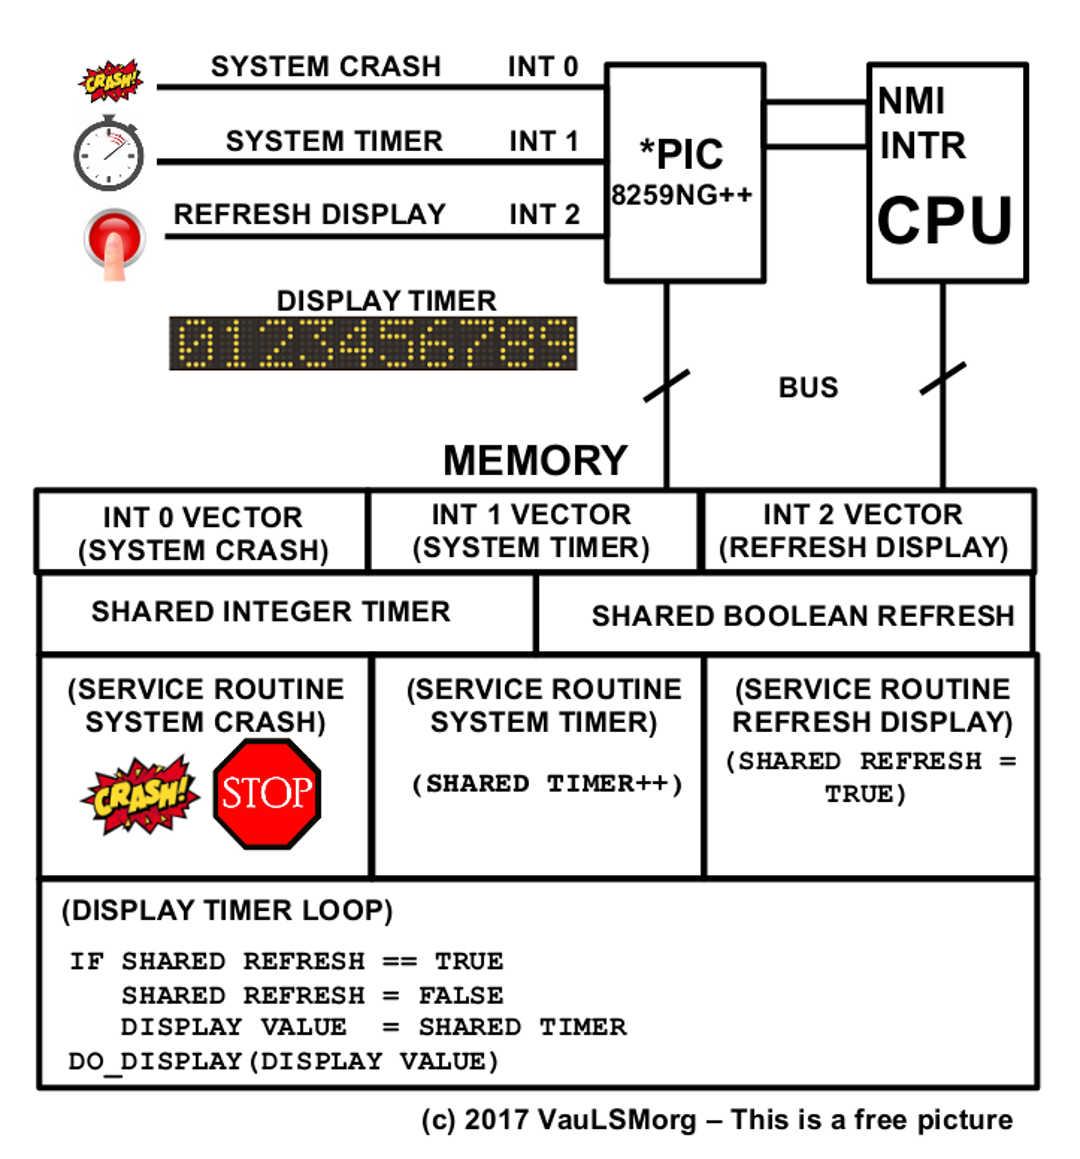
\includegraphics[width=0.56\linewidth]{os00-int-protection}
\caption{How to protect and secure this design?}
\end{figure}

\end{frame}

% XXXXXXXXXXXXXXXXXXXXXXXXXXXXXXXXXXXXXXXXXXXXXXXXXXXXXXXXXXXXXXXXXXXXXXXXXX
\section{The Security Problem}
\begin{frame}[fragile]
\frametitle{The Security Problem}
\begin{itemize}
\item \textbf{OSC10}:
\begin{itemize}
\item \textbf{Security} is a measure of confidence that the integrity of 
      a system and its data will be preserved.
\item \textbf{Protection} is the set of mechanisms that control the access
      of processes and users to the resources defined by a computer system.
\end{itemize}
\item Secure System, Intruders, Threat, Attack.
\item Security Violation Categories: Breach of (confidentiality, integrity, 
      availability), theft of service, DOS.
\item Security Violation Methods: Masquerading, Replay attack, 
      Human-in-the-middle attack, Session hijacking, Privilege escalation.
\item Security Measure Levels: Physical, Network, Operating System, Application. 
\item Program, System, and Network Threats
\begin{itemize}
\item Social Engineering: Phishing.
\item Security Hole: Code Review.
\item Principle of least privilege.
\end{itemize}
\end{itemize}
\end{frame}

% 15 XXXXXXXXXXXXXXXXXXXXXXXXXXXXXXXXXXXXXXXXXXXXXXXXXXXXXXXXXXXXXXXXXXXXXXX
% XXXXXXXXXXXXXXXXXXXXXXXXXXXXXXXXXXXXXXXXXXXXXXXXXXXXXXXXXXXXXXXXXXXXXXXXXX
\begin{frame}[fragile]
\frametitle{The Security Problem (cont)}
\begin{itemize}
\item Threats: Malware, Trojan Horse, Spyware, Ransomware, Trap (back) Door,
      Logic Bomb, Code-injection Attack, Overflow, Script Kiddie.
\item Viruses: Virus Dropper, Virus Signature, Keystroke Logger.
\item Worm, Sniffing, Spoofing, Port Scanning, DOS (Denial of Service).
\item Cryptography: (Symmetric and Asymmetric) Encryption, Public/Private Key Pairs,
      Key Distribution, Digital Certificate.
\item User Authentication: 
\begin{itemize}
\item Password: One Time Password, Two-Factor Authentication,
\item Biometrics.
\end{itemize}
\item Implementing Security Defenses: Policy, Assesment, Prevention, Detection, Protection, Auditing.
\item Linux Security
\item gnupg \& sha1sum
\end{itemize}
\end{frame}

% XXXXXXXXXXXXXXXXXXXXXXXXXXXXXXXXXXXXXXXXXXXXXXXXXXXXXXXXXXXXXXXXXXXXXXXXXX
\section{Protection}
\begin{frame}[fragile]
\frametitle{Protection}
\begin{itemize}
\item Principle of Least Privilege
\item Domain Structure and Access Matrix
\item ACL: Access Control List
\begin{itemize}
\item Domain = set of Access-rights (eg. \textbf{user-id}).
\item Access-right = <object-name, rights-set> (eg. object: file).
\end{itemize}
\begin{tabular}{| l | c | c | c | c |}
\hline
\makebox[9mm]{} & \makebox[9mm]{File1} & \makebox[9mm]{File2} & \makebox[9mm]{File3} & \makebox[9mm]{Printer} \\
\hline
User1 & Read  &       & Read    &         \\
\hline
User2 &       &       &         & Print   \\
\hline
User3 &       & Read  & Execute & Print   \\
\hline
User4 & R/W   &       & R/W     & Print   \\
\hline
\end{tabular}
\item Access-right Plus Domain (Users) as Objects
\begin{tabular}{| l | c | c | c | c | c | c | c | c | c |}
\hline
   & F1  & F2 & F3   & Printer & U1 & U2 & U3 & U4 \\
\hline
U1 & R   &    & R    &         &    & SW &    &    \\
\hline
U2 &     &    &      & Print   &    &    & SW & SW \\
\hline
U3 &     & R  & EXEC & Print   &    &    &    &    \\
\hline
U4 & R/W &    & R/W  & Print   & SW &    &    &    \\
\hline
\end{tabular}

\end{itemize}

\end{frame}

% XXXXXXXXXXXXXXXXXXXXXXXXXXXXXXXXXXXXXXXXXXXXXXXXXXXXXXXXXXXXXXXXXXXXXXXXXX
\begin{frame}
\frametitle{Copy Rights}
\begin{itemize}
\item Start

\begin{tabular}{| l | c | c | c | }
\hline
\makebox[9mm]{} & \makebox[9mm]{File1} & \makebox[9mm]{File2} & \makebox[9mm]{File3} \\
\hline
User1 & Exec &       & Write* \\
\hline
User2 & Exec & Read* & Exec   \\
\hline
User3 & Exec &       &         \\
\hline
\end{tabular}

\item User3: Read access to File2 (by User2)

\begin{tabular}{| l | c | c | c | }
\hline
\makebox[9mm]{} & \makebox[9mm]{File1} & \makebox[9mm]{File2} & \makebox[9mm]{File3} \\
\hline
User1 & Exec &       & Write* \\
\hline
User2 & Exec & Read* & Exec   \\
\hline
User3 & Exec & \textbf{Read} &         \\
\hline
\end{tabular}

\item Owner Rights

\begin{tabular}{| l | c | c | c | }
\hline
\makebox[9mm]{} & \makebox[9mm]{File1} & \makebox[9mm]{File2} & \makebox[9mm]{File3} \\
\hline
User1 & O \& E &       & W \\
\hline
User2 & & O \& R* \& W* & O \& R* \& W   \\
\hline
User3 &  & W & W         \\
\hline
\end{tabular}

\end{itemize}

\end{frame}

% XXXXXXXXXXXXXXXXXXXXXXXXXXXXXXXXXXXXXXXXXXXXXXXXXXXXXXXXXXXXXXXXXXXXXXXXXX
\section{Privacy}
\begin{frame}[fragile]
\frametitle{Privacy (Wikipedia)}
\begin{itemize}
\item Privacy can mean different things in different contexts; different people, 
      cultures, and nations have different expectations about how much privacy 
      a person is entitled to or what constitutes an invasion of privacy.
\item Considering all discussions as one of these concepts
\begin{itemize}
\item Right to be let alone (such as one's own home).
\item Limited access (no information collection).
\item Control over information (in the era of big data).
\item States of privacy: solitude, intimacy, anonymity, and reserve.
\item Secrecy: does not apply for any already publicly disclosed.
\item Personhood and autonomy.
\item Self-identity and personal growth.
\end{itemize}
\end{itemize}
\end{frame}

% XXXXXXXXXXXXXXXXXXXXXXXXXXXXXXXXXXXXXXXXXXXXXXXXXXXXXXXXXXXXXXXXXXXXXXXXXX
\begin{frame}[fragile]
\frametitle{Beginner's Guide to Internet Safety \& Privacy}
\begin{itemize}
\item \textbf{URL:} \url{https://choosetoencrypt.com/privacy/complete-beginners-guide-to-internet-safety-privacy/}
\item Who Are You Protecting Yourself From?
\begin{itemize}
\item Governments
\item ISPs
\item (H)Crackers
\item Trackers
\item Advertisers/Malwertisers
\end{itemize}
\item Which Information Should You Keep Private?
\begin{itemize}
\item Metadata
\item Personal Information
\item Passwords
\item Financial Data
\item Medical Records
\item History
\item Communication
\end{itemize}
\end{itemize}
\end{frame}

% XXXXXXXXXXXXXXXXXXXXXXXXXXXXXXXXXXXXXXXXXXXXXXXXXXXXXXXXXXXXXXXXXXXXXXXXXX
\section{C Language}
\begin{frame}
\frametitle{C Language}
\begin{itemize}
\item Reference: (Any C Language Tutorial)
\item Visit
\url{https://github.com/UI-FASILKOM-OS/SistemOperasi/tree/master/Demos/Week02/c-language}
\end{itemize}
\end{frame}

% XXXXXXXXXXXXXXXXXXXXXXXXXXXXXXXXXXXXXXXXXXXXXXXXXXXXXXXXXXXXXXXXXXXXXXXXXX
\section{Week 02: Summary}
\begin{frame}
\frametitle{Week 02: Summary}
\begin{itemize}
\item Reference: (OSC10-ch16 OSC10-ch17 demo-w02)
\item Goals of Protection
\item Domain and Access Matrix
\item ACL: Access Control List
\item The Security Problem
\item Threats: Trojan Horse, Trap Door, Overflow, Viruses, Worms, Port Scanning, 
      DOS (Denial of Service).
\item Cryptography: (Symmetric and Asymmetric) Encryption,
\item User Authentication: Password, Biometrics.
\item Implementing Security Defenses: Policy, Assesment, Prevention, Detection, Protection, Auditing.
\item Privacy.
\end{itemize}
\end{frame}

% XXXXXXXXXXXXXXXXXXXXXXXXXXXXXXXXXXXXXXXXXXXXXXXXXXXXXXXXXXXXXXXXXXXXXXXXXX

% %%%%%%%%%%%%%%%%%%%%%%%%%%%%%%%%%%%%%%%%%%%%%%%%%%%%%%%%%%%%%%%%%%%%%%%
% Beamer Presentation - LaTeX - Template Version 1.0 (10/11/12)
% This template has been downloaded from: http://www.LaTeXTemplates.com
% License: % CC BY-NC-SA 3.0 (http://creativecommons.org/)
% Modified by Rahmat M. Samik-Ibrahim

% REV347 Sat 18 Sep 2021 16:27:41 WIB
% REV324 Mon 09 Aug 2021 21:58:27 WIB
% REV309 Mon 05 Jul 2021 15:32:10 WIB
% REV285 Sat 13 Mar 2021 06:25:04 WIB
% REV280 Tue 09 Mar 2021 07:06:04 WIB
% STARTX Sun Sep 13 08:49:47 WIB 2020
% %%%%%%%%%%%%%%%%%%%%%%%%%%%%%%%%%%%%%%%%%%%%%%%%%%%%%%%%%%%%%%%%%%%%%%%%

% XXXXXXXXXXXXXXXXXXXXXXXXXXXXXXXXXXXXXXXXXXXXXXXXXXXXXXXXXXXXXXXXXXXXXXXXXX
\section{Week 02: Check List}
\begin{frame}
\frametitle{Week 02: Check List (Deadline: 19 Sep 2021).}
\begin{itemize}
\item [$\square$] Week 02: Assignment (\href{https://os.vlsm.org/Slides/os02.pdf}{\textbf{os02.pdf}}).
(Eg. \textbf{cbkadal}).
\begin{itemize}
\item Visit \url{https://osp4diss.vlsm.org/\#idx07}
\begin{enumerate}
\item \href{https://www.os-book.com/OS10/slide-dir/}{Read OSC10 chapter 16 + chapter 17}
\item Try Demos in {\tiny \url{https://github.com/UI-FASILKOM-OS/SistemOperasi/tree/master/Demos/}}.
\item Watch: \href{https://youtu.be/rcDO8km6R6c}{Cyber Security Introduction part 1} and 
\href{https://youtu.be/CivG_2UqKMg}{the begining of part 2}.
\item Generate a GnuPG Key Pair {\tiny \url{https://osp4diss.vlsm.org/CBKadal2.html}}.
\item List of all GnuPG Keys {\tiny \url{https://osp4diss.vlsm.org/W02-01.html}}.
\item Importing \textbf{ospubkey.txt Key} from 
      {\tiny \url{https://osp4diss.vlsm.org/W02-02.html}}.
\item \href{https://osp4diss.vlsm.org/W02-03.html}{Signing the Operating Systems public key (Optional)}.
\item \href{https://osp4diss.vlsm.org/W02-04.html}{Export \textbf{YOUR PUBLIC KEY} to your repo file ''TXT/mypubkey.txt''}. 
\item \href{https://cbkadal.github.io/os212/LINKS/}{Update your bookmark links. See C.B. Kadal's ''LINKS/''}
\item \href{https://osp4diss.vlsm.org/W02-05.html}{Review your peer links}.
\item Write (or copy) a simple and useful \texttt{bash} script (\url{https://cbkadal.github.io/os212/TXT/myscript.sh}).
\item \href{https://cbkadal.github.io/os212/TXT/mylog.txt}{Update your log. See C.B. Kadal's ''mylog.txt''}
\item \href{https://osp4diss.vlsm.org/W02-06.html}{Run "myscript.sh" script to generate SHA256SUM and SHA256SUM.asc}.
\end{enumerate}
\end{itemize}
\end{itemize}
\end{frame}



% 12 XXXXXXXXXXXXXXXXXXXXXXXXXXXXXXXXXXXXXXXXXXXXXXXXXXXXXXXXXXXXXXXXXXXXXXX
% XXXXXXXXXXXXXXXXXXXXXXXXXXXXXXXXXXXXXXXXXXXXXXXXXXXXXXXXXXXXXXXXXXXXXXXXXX
\section{The End}
\begin{frame}
\frametitle{The End}
\begin{itemize}
\item[$\square$] This is the end of the presentation.
\item[$\boxtimes$] This is the end of the presentation.
\item This is the end of the presentation.
\end{itemize}
\end{frame}

% XXXXXXXXXXXXXXXXXXXXXXXXXXXXXXXXXXXXXXXXXXXXXXXXXXXXXXXXXXXXXXXXXXXXXXXXXX
\end{document}

